%!TEX program = xelatex
%!BIB program = bibtex
%!TEX root = ../main.tex
% ----- CONFIGURAÇÕES ----- %
\documentclass[12pt]{article}
\usepackage{graphicx} % imagens
\usepackage[brazil]{babel} % idioma
\usepackage{amsmath} % equações
\numberwithin{equation}{section} % numeração de equação numero-da-secao.numero-da-equacao
\usepackage{caption} % legenda em imagens e tabelas
\usepackage{subcaption} % legenda em subimagens e subtabelas
\newcommand{\source}[1]{\caption*{Fonte: {#1}} } % para adicionar fonte de imagens e tabelas
\usepackage{enumitem} % criação de listas
\usepackage{cite} % para citar seções, imagens...
\usepackage[hidelinks]{hyperref} % para ter itens (citação de seções, sumário...) clicáveis
\usepackage{indentfirst} % espaçamento do primeiro parágrafo
%\setcounter{section}{0} % começa as seções em 0
\usepackage{booktabs}
% --- ABNT --- %
% definindo fonte
\usepackage{fontspec}
\setmainfont{Times New Roman}
% tamanho da folha e margens
\usepackage[a4paper, left=3cm, top=3cm, right=2cm, bottom=2cm]{geometry}
% definindo tamanho para items e subitems
\usepackage{titlesec}
\titleformat{\section}{\normalfont\fontsize{16}{15}\bfseries}{\makebox[25pt][l]{\thesection}}{0pt}{}
\titleformat{\subsection}{\normalfont\fontsize{16}{15}\bfseries}{\makebox[25pt][l]{\thesubsection}}{0pt}{}
% para configurar alinhamento e espaçamento
\usepackage{setspace}
\usepackage{ragged2e}
\titlespacing*{\section}{0.75cm}{12pt}{12pt}
\titlespacing*{\subsection}{0.75cm}{12pt}{12pt}
\usepackage[num]{abntex2cite} % bibliografia e citação no padrão ABNT
\usepackage{mathtools}

\usepackage{blindtext} % pacote para geração de texto aleatório, pode ser removido
\usepackage{float}
\begin{document}

% ---- Renomeando títulos do sistema para português ---- %
\renewcommand*\contentsname{Sumário}
\renewcommand{\listfigurename}{Lista de Ilustrações}
\renewcommand{\listtablename}{Lista de Tabelas}
\renewcommand{\refname}{}

\onehalfspace % espaçamento entrelinhas 1.5
\justifying % alinhamento justificado
\setlength{\leftskip}{0.75cm} % corpo do texto a 0.75 cm da margem esquerda
\graphicspath{{./imagens/}} % pasta com imagens
\begin{titlepage}
    \begin{center}
        Escola Politécnica da Universidade de São Paulo\\
        Departamento de Engenharia de Sistemas \\ PTC3567 – Ciência de Dados em Automação e Engenharia

        \vspace{1.5cm}
        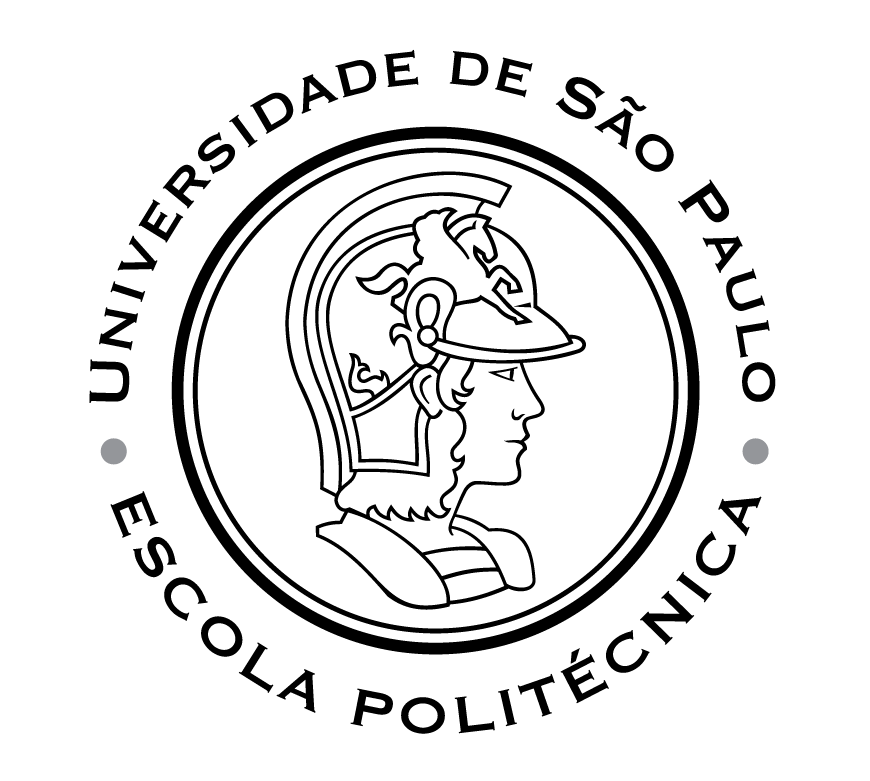
\includegraphics[width=0.4\textwidth]{Poli.png}
        
        \vspace*{1.5cm}
        \fontsize{18}{15}\textbf{Relatório Final - PTC3567}
        
        %\vspace*{1.5cm}
        %Estágio em Deal Management na Mastercard

        \vspace*{1.5cm}
        \begin{tabular}{c c}
	        Mariana Aquino Rocha & 13680251 \\
            Lucas Parisotto Fabre &  18005349 \\
            Roberto Machado e Silva Gomide & 11321371
        \end{tabular}
        
        \vspace*{\fill}
        {São Paulo\\
        Agosto de 2026}
    \end{center}
\end{titlepage}

\newpage\textit{\textbf{Resumo: }até 250 palavras}

\textit{Palavras-chave: 3 palavras}
\newpage\textit{\textbf{Abstract: }maximum of 250 words}

\textit{Key-words: 3 words}
\newpage\listoffigures
\newpage\listoftables
\newpage\tableofcontents

\newpage\section{INTRODUÇÃO} \label{sec:intro}

Esta seção definirá o problema tratado, além de apontar experimentos semelhantes que ajudarão o grupo a desenvolver este trabalho.

\subsection{Problema}

A figura \label{fig:canvas} elabora os principais pontos tratados neste projeto de ciência de dados.

\begin{figure}[H]
    \centering
    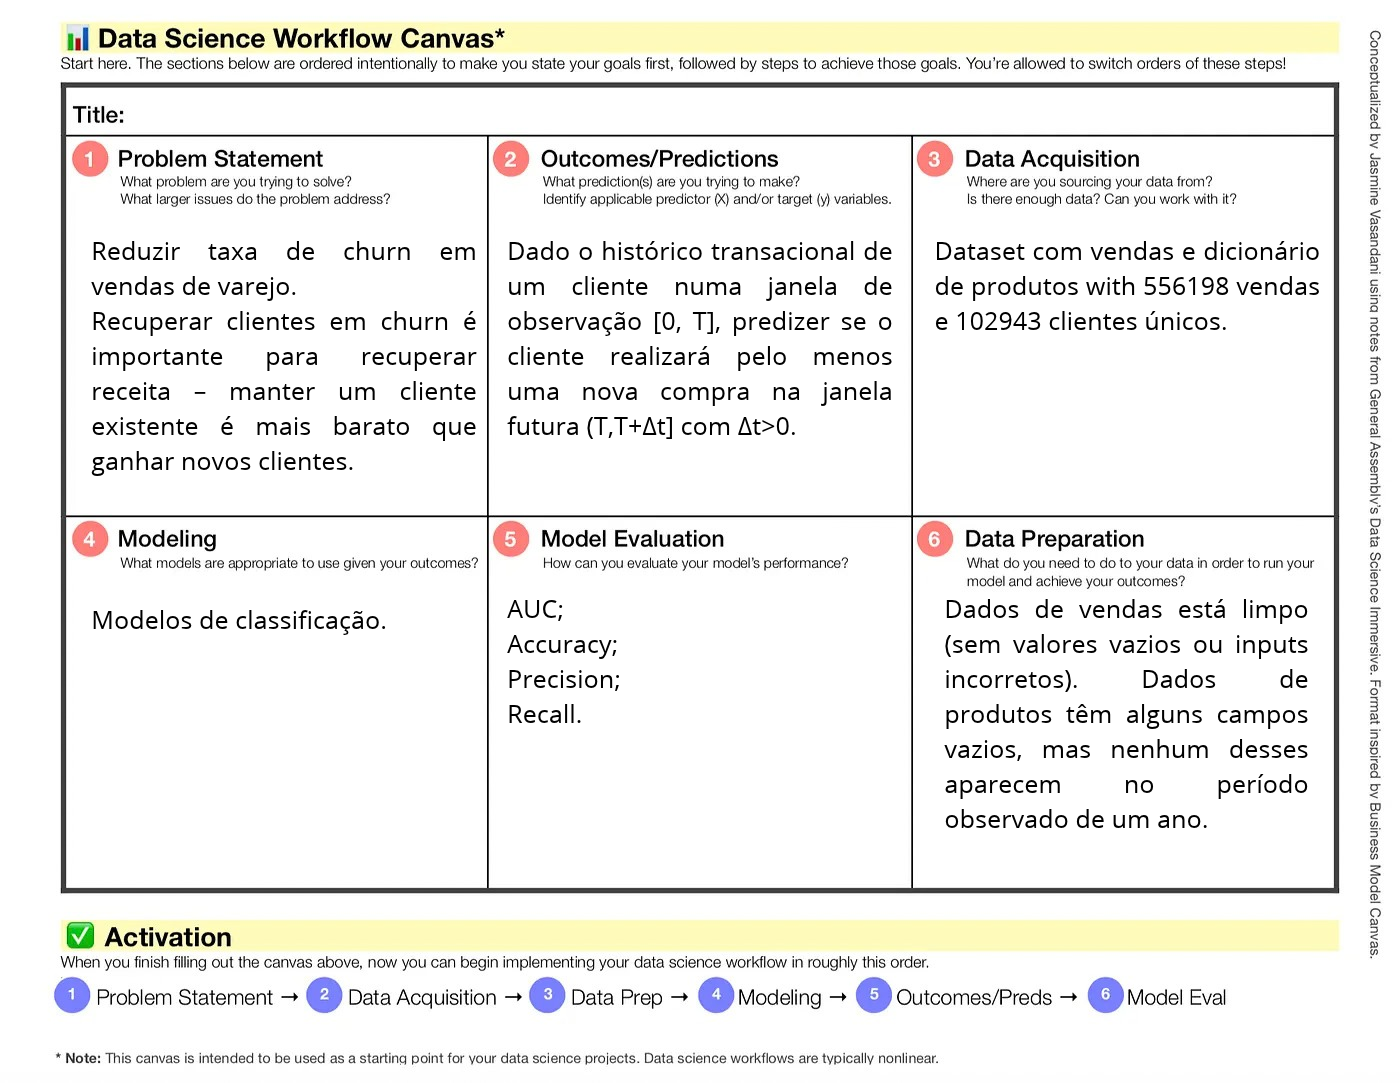
\includegraphics[width=1\linewidth]{imagens/canva2.png}
    \caption{Canvas para o projeto}
    \label{fig:canvas}
\end{figure}

De uma perspectiva de negócios, o problema é de previsão de churn: dado o histórico transacional de um cliente em uma janela de observação passada, é possível prever se o cliente realizará uma transação no futuro, ou se desengajará da loja?

O \textit{dataset} utilizado foi disponibilizado pelo mentor do grupo e traz dados de vendas de uma loja varejista.

\subsection{Artigos e experimentos semelhantes}

Teste
\newpage\section{ESTRATÉGIAS DE GESTÃO DOS DADOS}\label{sec:conteudo1}
\blindtext
\subsection{Titulo da Subsecao}\label{subsec:conteudo1}

\noindent\textbf{\textit{Titulo da subsubsecao 1}}



\newpage\section{CARACTERIZAÇÃO E PREPARAÇÃO DOS DADOS}\label{sec:conteudo2}

Esta seção se destina a analisar os metadados do \textit{dataset} fornecido, avaliar a qualidade deste e a realizar uma análise exploratória de dados (EDA) inicial, fonte das hipóteses a serem testadas na modelagem.

\subsection{Caracterização dos Dados}\label{subsec:caracterizacao}

\subsubsection{Visão Geral e Metadados}
O conjunto de dados utilizado neste projeto provém do histórico transacional de vendas de uma rede varejista, complementado por um catálogo cadastral de produtos. 

A base principal de vendas (\texttt{vendas.csv}) registra o fluxo transacional ao longo de todo o ano de 2024 (período de 01 de janeiro a 31 de dezembro de 2024). Essa base é composta por \textbf{556.198 registros} e contempla \textbf{102.943 clientes únicos}, devidamente anonimizados via identificadores alfanuméricos. 
A granularidade dos dados ocorre ao nível de item faturado: cada linha da tabela corresponde a um produto específico adquirido em um determinado atendimento.
Cada venda corresponde a um único produto, e várias vendas podem ocorrer num mesmo atendimento.

A base auxiliar de produtos (\texttt{produto.csv}) conta originalmente com 6.500 mercadorias cadastradas, das quais são herdadas as classificações de categorias e subcategorias após o cruzamento via identificador único do produto (\textit{Stock Keeping Unit} -- SKU).

\subsubsection{Dicionário de Dados}
A Tabela~\ref{tab:dicionario_dados} descreve os atributos disponíveis, sua tipagem original e a respectiva descrição de negócio.


\begin{table}[H]
\centering
\caption{Dicionário de variáveis da base de vendas e catálogo de produtos}
\label{tab:dicionario_dados}
\begin{tabular}{llp{9.5cm}}
\toprule
\textbf{Atributo} & \textbf{Tipo} & \textbf{Descrição} \\
\midrule
\texttt{COD\_ATEND}    & Texto       & Código identificador do atendimento. \\
\texttt{COD\_VENDA}    & Texto       & Código identificador da venda. \\
\texttt{COD\_FILIAL}   & Inteiro     & Código identificador da loja em que o atendimento foi realizado. \\
\texttt{FILIAL}        & Texto       & Tipo de filial (Rua ou Shopping)/ \\
\texttt{DATA\_ATEND}   & Data/Hora   & Data de atendimento daquele cliente a respeito daquele produto. \\
\texttt{SKU}           & Inteiro     & Código do produto. \\
\texttt{UNID}          & Texto       & Unidade de comercialização do item (ex.: UN, KG). \\
\texttt{QTD\_VENDA}    & Numérico    & Quantidade vendida do produto. \\
\texttt{FATUR\_VENDA}  & Numérico    & Faturamento bruto gerado pelo item em reais (R\$). \\
\texttt{CLI\_CPF}      & Texto       & Código do cliente. \\
\texttt{NOME\_PRODUTO} & Texto       & Descrição do produto \\
\texttt{CATEGORIA}     & Texto       & Categoria do produto. \\
\texttt{SUBCATEGORIA}  & Texto       & Subcategoria do produto. \\
\bottomrule
\end{tabular}
\source{Elaborado pelos autores.}
\end{table}

\subsubsection{Estatísticas Descritivas}
Para as variáveis numéricas transacionais contínuas (\texttt{QTD\_VENDA} e \texttt{FATUR\_VENDA}), foram calculadas as métricas de tendência central, dispersão e quartis, sumarizadas na Tabela~\ref{tab:estatisticas_descritivas}.

\begin{table}[H]
\centering
\caption{Estatísticas descritivas das variáveis quantitativas da base de vendas}
\label{tab:estatisticas_descritivas}
\begin{tabular}{lrrrrrr}
\toprule
\textbf{Variável} & \textbf{Média} & \textbf{Desv. Pad.} & \textbf{Mínimo} & \textbf{Mediana} & \textbf{Q3 (75\%)} & \textbf{Máximo} \\
\midrule
\texttt{QTD\_VENDA}        & 0,28  & 0,52  & 0,002 & 0,15 & 0,27  & 100,70 \\
\texttt{FATUR\_VENDA} (R\$) & 14,11 & 29,04 & 0,03  & 7,82 & 14,26 & 4.994,76 \\
\bottomrule
\end{tabular}
\source{Elaborado pelos autores.}
\end{table}

Observa-se acentuada assimetria à direita na distribuição do faturamento por item (\texttt{FATUR\_VENDA}), onde a média (R\$~14,11) é substancialmente superior à mediana (R\$~7,82), havendo valores pontuais de até R\$~4.994,76, típicos de compras atípicas ou itens de maior valor agregado. Em relação a \texttt{QTD\_VENDA}, a mediana em 0,15 e percentis fracionários evidenciam a forte presença de produtos comercializados por peso ou a granel (quilograma).
\subsection{Preparação e Qualidade dos Dados}\label{subsec:preparacao}

\subsubsection{Diagnóstico de Qualidade e Valores Ausentes}
Antes de iniciar as análises estatísticas e a engenharia de atributos, foi conduzida uma auditoria de integridade sobre as bases de dados para identificar valores nulos ou registros corrompidos.

\begin{itemize}[leftmargin=*]
    \item \textbf{Base de Vendas (\texttt{vendas.csv}):} Apresentou integridade completa em todas as 556.198 linhas. Nenhum dos dez atributos continha valores ausentes (\textit{nulls}) ou campos não preenchidos.
    \item \textbf{Base de Produtos (\texttt{produto.csv}):} Identificou-se que, dos 6.500 produtos catalogados, 2.001 registros não possuíam informação preenchida nos campos \texttt{CATEGORIA} e \texttt{SUBCATEGORIA}, além de 1 registro com \texttt{SKU} nulo. Contudo, ao realizar a junção à esquerda (\textit{left join}) com a base transacional de vendas, constatou-se que \textbf{nenhum desses produtos incompletos foi comercializado no período de 2024}. O conjunto resultante do cruzamento conteve 100\% de preenchimento para todas as mercadorias vendidas, dispensando o preenchimento manual ou correção desses produtos com preenchimento incorreto.
\end{itemize}

\subsubsection{Adequação de Tipos e Tratamento Temporal}
Para viabilizar as análises temporais e de comportamento de compra, foram realizados os seguintes ajustes de formatação e tipagem:
\begin{enumerate}[leftmargin=*]
    \item \textbf{Conversão Temporal:} O campo \texttt{DATA\_ATEND}, originalmente importado no formato textual (\textit{string}), foi convertido para o tipo de dado temporal nativo (\texttt{datetime64}), permitindo operações como ordenação cronológica, extração de sazonalidade mensal e cálculo de diferenças temporais entre transações consecutivas.
    \item \textbf{Semântica de Identificadores:} Variáveis codificadas numericamente como \texttt{COD\_FILIAL} e \texttt{SKU} foram formalmente tratadas como atributos categóricos nominais/identificadores, evitando que operações aritméticas inválidas de média ou soma fossem aplicadas a esses códigos.
\end{enumerate}

\subsubsection{Tratamento de Granularidade e Agrupamentos}
Como a base original registra cada item de venda individualmente, um mesmo atendimento (\texttt{COD\_ATEND}) pode conter múltiplas linhas associadas à mesma data (\texttt{DATA\_ATEND}) e cliente (\texttt{CLI\_CPF}). 

Para o estudo de recorrência e cálculo do intervalo entre compras, realizou-se a consolidação das compras no nível de \textbf{visita do cliente}, agrupando por \texttt{CLI\_CPF} e \texttt{DATA\_ATEND}. Adotou-se a premissa de que o dia é a unidade de visitação básica do consumidor à rede varejista, eliminando duplicidades de múltiplos itens faturados em uma mesma ida à loja.

\subsection{Análise Exploratória de Dados (EDA) e Teste de Hipóteses}\label{subsec:eda}

Com os dados higienizados e agrupados no nível de visita diária por cliente (totalizando 297.257 visitas únicas ao longo de 2024), conduziu-se a Análise Exploratória de Dados estruturada em torno da definição empírica do ciclo de recompra e da validação de cinco hipóteses de negócio que nortearam a engenharia de atributos da modelagem.

\subsubsection{Ciclo de Recompra e Definição Empírica da Janela de \textit{Churn}}
Inicialmente, constatou-se que, dos 102.943 clientes únicos atendidos em 2024, \textbf{50,20\% (51.678 consumidores)} realizaram apenas uma única visita no ano (\textit{one-timers}), enquanto \textbf{49,80\% (51.265 consumidores)} apresentaram comportamento de recompra (\textit{recurring}), sendo responsáveis por 245.579 visitas.

Para determinar a partir de quantos dias de inatividade um consumidor pode ser considerado em evasão (\textit{churn}), calculou-se a diferença temporal em dias entre visitas consecutivas de todos os clientes recorrentes ($N = 194.314$ intervalos entre compras). Os quantis da distribuição do tempo entre visitas revelaram um padrão bem definido:
\begin{itemize}[leftmargin=*]
    \item \textbf{1º Quartil (25\%):} 14,0 dias (ciclo quinzenal de reposição);
    \item \textbf{Mediana (50\%):} 29,0 dias (ciclo tipicamente mensal);
    \item \textbf{3º Quartil (75\%):} 63,0 dias (ciclo bimestral);
    \item \textbf{Percentil 90\%:} 119,0 dias.
\end{itemize}

Observou-se que \textbf{83,88\% de todas as recompras da rede ocorrem em até 90 dias (3 meses)} após a visita anterior. Caso um cliente ultrapasse 90 dias sem retornar à loja, a probabilidade empírica de retorno espontâneo cai drasticamente. Esse resultado fundamentou estatisticamente a adoção da \textbf{janela de 90 dias (3 meses)} como critério oficial para a definição da variável resposta (\texttt{flag\_churn}) na etapa de modelagem.

\subsubsection{H1: Clientes de Passagem (\textit{One-Timers}) vs. Clientes Desengajados}
A primeira hipótese investigou se o grupo de clientes inativos há mais de 90 dias no encerramento do ano (corte em \texttt{02/10/2024}, totalizando 54.985 clientes em \textit{churn}) é composto majoritariamente por compradores ocasionais de visita única ou por clientes fiéis que abandonaram a marca.
\begin{itemize}[leftmargin=*]
    \item \textbf{Clientes de Passagem (\textit{One-Timers} em \textit{churn}):} 36.802 consumidores (\textbf{66,93\%} do total em \textit{churn});
    \item \textbf{Clientes Recorrentes Desengajados ($\ge 2$ visitas em \textit{churn}):} 18.183 consumidores (\textbf{33,07\%} do total em \textit{churn}).
\end{itemize}
A hipótese \textbf{H1 foi confirmada}: dois terços da evasão bruta decorrem da falha na conversão da primeira para a segunda compra, justificando a criação de variáveis explícitas de quantidade de visitas (\texttt{qtde\_visitas}) e meses de ativação (\texttt{qtd\_mes\_ativacao}) no modelo preditivo.

\subsubsection{H2.1: Aumento Progressivo do Intervalo entre Visitas antes do \textit{Churn}}
Avaliou-se a hipótese de que clientes recorrentes apresentariam um espaçamento gradualmente maior entre suas três últimas compras (\texttt{antepenultimo\_intervalo}, \texttt{penultimo\_intervalo} e \texttt{ultimo\_intervalo}) antes de entrarem em \textit{churn}. A comparação entre clientes ativos (\texttt{churn = False}) e evadidos (\texttt{churn = True}) com ao menos quatro visitas registradas é apresentada na Tabela~\ref{tab:eda_intervalos}.

\begin{table}[H]
\centering
\caption{Evolução das médias e medianas dos três últimos intervalos entre compras (em dias)}
\label{tab:eda_intervalos}
\begin{tabular}{lrrrrrr}
\toprule
& \multicolumn{3}{c}{\textbf{Média do Intervalo (dias)}} & \multicolumn{3}{c}{\textbf{Mediana do Intervalo (dias)}} \\
\cmidrule(lr){2-4} \cmidrule(lr){5-7}
\textbf{Status no Fim do Ano} & \textbf{Antepenúlt.} & \textbf{Penúlt.} & \textbf{Último} & \textbf{Antepenúlt.} & \textbf{Penúlt.} & \textbf{Último} \\
\midrule
Ativo (\texttt{churn = False}) & 48,3 & 48,5 & 50,6 & 33,0 & 34,0 & 36,0 \\
Em Evasão (\texttt{churn = True}) & 41,6 & 41,6 & 47,3 & 31,0 & 32,0 & 36,0 \\
\bottomrule
\end{tabular}
\source{Elaborado pelos autores.}
\end{table}

Constatou-se que as medianas evoluem de forma praticamente idêntica nos dois grupos ($33 \rightarrow 34 \rightarrow 36$ dias nos ativos contra $31 \rightarrow 32 \rightarrow 36$ dias nos evadidos), e a proporção de clientes cujo intervalo aumentou antes da última compra foi semelhante (54\% no grupo em \textit{churn} contra 51\% nos ativos). Logo, a hipótese \textbf{H2.1 foi refutada}, demonstrando que a perda de ritmo isolada entre visitas consecutivas não discrimina a evasão, sendo mais eficaz utilizar a recência absoluta até a data de referência (\texttt{qtd\_dias\_ultima\_compra}) e a média global de compras por mês (\texttt{avg\_compras\_mes}).

\subsubsection{H2.2: Influência da Categoria de Produto na Fidelização e Recorrência}
Cruzando a base transacional com o catálogo de produtos (\texttt{CATEGORIA}), investigou-se se o perfil da cesta adquirida impacta a retenção do consumidor. A Tabela~\ref{tab:eda_categorias} sumariza o alcance de clientes únicos, a taxa de recorrência (proporção de compradores da categoria que realizaram mais de uma visita no ano), a taxa de \textit{churn} no último trimestre e o faturamento anual por categoria.

\begin{table}[H]
\centering
\caption{Desempenho de retenção, recorrência e faturamento anual por categoria de produto}
\label{tab:eda_categorias}
\resizebox{\textwidth}{!}{%
\begin{tabular}{lrrrr}
\toprule
\textbf{Categoria de Produto} & \textbf{Clientes Únicos} & \textbf{Taxa de Recorrência (\%)} & \textbf{Taxa de \textit{Churn} (\%)} & \textbf{Faturamento Anual (R\$)} \\
\midrule
Castanhas \& Oleaginosas       & 30.615 & 69,5\% & 42,1\% & 1.663.514,00 \\
Bacalhau \& Pescados           & 13.511 & 61,2\% & 25,6\% & 1.486.920,00 \\
Temperos \& Condimentos        & 55.445 & 62,0\% & 48,6\% &   940.771,64 \\
Frutas                         & 28.486 & 71,9\% & 38,2\% &   932.519,00 \\
Mixes da Casa                  & 16.624 & 67,8\% & 44,3\% &   445.741,95 \\
Grãos                          & 21.538 & 72,4\% & 42,3\% &   375.510,20 \\
Superalimentos \& Energéticos  & 10.221 & 70,6\% & 42,8\% &   284.057,30 \\
Matinais                       & 17.781 & 74,4\% & 40,8\% &   227.005,13 \\
Aperitivos                     &  9.465 & 74,1\% & 40,2\% &   220.907,28 \\
Conservas                      &  5.732 & 76,0\% & 32,8\% &   138.752,75 \\
Lanchonete                     &  7.527 & 64,4\% & 49,0\% &   127.054,27 \\
Azeites \& Vinagres            &  2.777 & 75,2\% & 41,0\% &   105.960,17 \\
Ervas \& Chás                  &  7.015 & 69,0\% & 41,4\% &    98.113,84 \\
\bottomrule
\end{tabular}%
}
\source{Elaborado pelos autores.}
\end{table}

Os dados confirmam a hipótese \textbf{H2.2}: itens de reposição doméstica e rotina alimentar — como \textit{Conservas} (76,0\% de recorrência), \textit{Azeites \& Vinagres} (75,2\%), \textit{Matinais} (74,4\%), \textit{Grãos} (72,4\%) e \textit{Frutas} (71,9\%) — geram maior fidelização ao longo do ano. Em contrapartida, categorias de consumo imediato ou esporádico, como \textit{Lanchonete} (49,0\% de \textit{churn}) e \textit{Temperos \& Condimentos} (48,6\% de \textit{churn}), concentram maior proporção de clientes de passagem. Nota-se ainda que as seis maiores categorias em receita (\textit{Castanhas}, \textit{Bacalhau}, \textit{Temperos}, \textit{Frutas}, \textit{Mixes} e \textit{Grãos}) representam mais de 80\% do faturamento da rede, motivo pelo qual foram selecionadas para compor as variáveis setoriais do \textit{Book of Features}.

\subsubsection{H2.3: Sazonalidade Mensal e Efeito de Feriados}
Ao avaliar a evolução mensal do faturamento e do retorno de clientes ao longo dos 12 meses de 2024 frente ao número de feriados nacionais de cada mês, verificou-se correlação linear quase nula/negativa entre a quantidade de feriados e o volume de clientes recorrentes ($r = -0,121$), bem como correlação fraca com o faturamento mensal ($r = +0,108$). Meses sem nenhum feriado nacional (junho, julho e agosto) mantiveram fluxo elevado e crescente de retorno (entre 13.188 e 15.779 clientes recorrentes ativos). Os dois grandes picos de faturamento da rede ocorreram em \textbf{março} (R\$~839,3 mil, impulsionado pela Páscoa) e em \textbf{dezembro} (R\$~1,49 milhão, impulsionado pelas festas de fim de ano e venda de bacalhau/oleaginosas). Assim, a hipótese \textbf{H2.3 foi refutada}: o retorno de clientes não depende da quantidade de feriados do mês, mas sim de marcos sazonais gastronômicos específicos.

\subsubsection{H3: Comportamento por Tipo de Filial (\texttt{RUA}, \texttt{SHOPPING} e Híbrido)}
Por fim, testou-se a hipótese de que o formato físico da loja influencia o perfil de retenção. Os 102.943 clientes foram classificados em três grupos segundo seu histórico de visitação: exclusivos de lojas de \texttt{RUA}, exclusivos de lojas de \texttt{SHOPPING} e clientes multicanais (\texttt{Ambos / Híbrido}). Os resultados encontram-se na Tabela~\ref{tab:eda_filial}.

\begin{table}[H]
\centering
\caption{Comparativo de retenção, frequência e gasto médio anual por canal de atendimento}
\label{tab:eda_filial}
\resizebox{\textwidth}{!}{%
\begin{tabular}{lrrrrr}
\toprule
\textbf{Canal do Cliente} & \textbf{Total de Clientes} & \textbf{Taxa de \textit{Churn} (\%)} & \textbf{Taxa \textit{One-Timer} (\%)} & \textbf{Média Visitas/Ano} & \textbf{Gasto Médio Anual (R\$)} \\
\midrule
Exclusivo \texttt{SHOPPING} & 53.576 & 55,40\% & 54,69\% & 2,60 &  72,65 \\
Exclusivo \texttt{RUA}      & 47.200 & 52,07\% & 47,41\% & 3,12 &  77,73 \\
Ambos (Multicanal Híbrido)  &  2.167 & 33,41\% &  0,05\% & 5,05 & 132,79 \\
\bottomrule
\end{tabular}%
}
\source{Elaborado pelos autores.}
\end{table}

A hipótese \textbf{H3 foi confirmada}: lojas de \texttt{SHOPPING} atraem maior fluxo de passeio e compra por impulso (54,69\% de \textit{one-timers} e 55,40\% de \textit{churn}), enquanto lojas de \texttt{RUA} apresentam clientela mais recorrente (3,12 visitas/ano e menor \textit{churn} de 52,07\%). Destacam-se os clientes multicanais (que frequentam tanto Rua quanto Shopping), cuja taxa de \textit{churn} cai para apenas \textbf{33,41\%}, com frequência média de 5,05 visitas/ano e gasto anual 82\% superior (R\$~132,79). Essa evidência motivou a inclusão das variáveis de frequência e faturamento separadas por canal (\texttt{qtde\_visitas\_rua}, \texttt{qtde\_visitas\_shopping}, \texttt{fatur\_rua} e \texttt{fatur\_shopping}) no modelo preditivo.

\subsubsection{Síntese das Hipóteses Exploratórias}
A Tabela~\ref{tab:sintese_hipoteses_eda} consolida o veredito de cada hipótese testada na EDA e seu impacto direto na construção da modelagem subsequente.

\begin{table}[H]
\centering
\caption{Síntese dos testes de hipóteses da Análise Exploratória de Dados (EDA)}
\label{tab:sintese_hipoteses_eda}
\footnotesize
\begin{tabular}{p{2.8cm}p{4.5cm}cp{6.2cm}}
\toprule
\textbf{Hipótese} & \textbf{Enunciado} & \textbf{Veredito} & \textbf{Evidência Numérica Principal} \\
\midrule
Definição de \textit{Churn} & O \textit{churn} caracteriza-se após 90 dias sem compras. & \textbf{Confirmada} & Mediana de recompra de 29 dias; 83,88\% de todas as recompras ocorrem em até 90 dias. \\
\addlinespace
H1: Passagem vs. Desengajados & No grupo em \textit{churn} coexistem clientes de compra única e recorrentes desengajados. & \textbf{Confirmada} & 50,20\% da base geral é \textit{one-timer}; dentro do \textit{churn}, 66,93\% são \textit{one-timers} e 33,07\% são recorrentes. \\
\addlinespace
H2.1: Aumento do Intervalo & O intervalo entre compras aumenta progressivamente antes do \textit{churn}. & \textbf{Refutada} & Medianas dos 3 últimos intervalos praticamente iguais entre ativos ($33 \rightarrow 34 \rightarrow 36$d) e evadidos ($31 \rightarrow 32 \rightarrow 36$d). \\
\addlinespace
H2.2: Categorias de Rotina & Categorias de rotina doméstica geram maior fidelização que itens ocasionais. & \textbf{Confirmada} & Maior recorrência em Conservas (76\%), Azeites (75\%) e Matinais (74\%); maior \textit{churn} em Lanchonete (49\%) e Temperos (48,6\%). \\
\addlinespace
H2.3: Efeito Feriados & Meses com mais feriados apresentam maior retorno de clientes. & \textbf{Refutada} & Correlação levemente negativa ($r = -0,121$); meses sem feriados (jun--ago) tiveram alto retorno (13k--15k clientes). \\
\addlinespace
H3: Tipo de Filial & O canal (\texttt{SHOPPING} vs. \texttt{RUA}) influencia a retenção e a frequência. & \textbf{Confirmada} & Shopping tem maior \textit{churn} (55,4\%) e \textit{one-timers} (54,7\%); Rua tem maior frequência (3,12 vis./ano); Híbridos têm apenas 33,4\% de \textit{churn}. \\
\bottomrule
\end{tabular}
\source{Elaborado pelos autores.}
\end{table}
\newpage\section{MODELAGEM E ANÁLISE DOS DADOS}\label{sec:conteudo3}

Esta seção apresenta a estruturação dos dados para a predição de evasão de clientes (\textit{churn}), abrangendo a construção das variáveis explicativas, a definição das janelas temporais de observação e maturação, a divisão das bases de validação e a configuração dos modelos avaliados.

\subsection{Estruturação das Bases e Construção de Safras}\label{subsec:arquitetura_sql}

\subsubsection{Organização dos Dados}
Para organizar o processamento e separar os dados brutos da etapa de modelagem, os registros históricos de vendas e o catálogo de produtos foram consolidados em um banco de dados relacional. A estrutura foi dividida em três camadas:
\begin{enumerate}[leftmargin=*]
    \item \textbf{Base Transacional:} Contém o histórico original de vendas na granularidade de item comercializado por atendimento, cruzado com as informações cadastrais de categoria dos produtos.
    \item \textbf{Base de Atributos (\textit{Book of Features}):} Reúne os indicadores comportamentais agregados por cliente para cada data de referência mensal (\texttt{dt\_ref}), sem incluir a variável resposta.
    \item \textbf{Tabela Analítica de Modelagem (ABT):} Resulta do cruzamento entre a base de atributos e o histórico de compras nos meses subsequentes à data de referência, atribuindo a cada cliente o rótulo de evasão (\texttt{flag\_churn}).
\end{enumerate}

\subsubsection{Engenharia de Atributos e Janela de Observação}
A construção das variáveis explicativas baseia-se em fotografias mensais (\textit{snapshots}), definidas sempre no primeiro dia de cada mês (\texttt{dt\_ref}). Para cada data de referência, são consideradas as transações realizadas pelo cliente nos \textbf{6 meses imediatamente anteriores}:
\begin{equation}
    \texttt{DATA\_ATEND} \in \big[\text{date}(\texttt{dt\_ref}, \text{`-6 months'}), \; \texttt{dt\_ref}\big)
\end{equation}
De forma complementar, consulta-se todo o histórico anterior a \texttt{dt\_ref} para calcular o tempo total de relacionamento do cliente com a rede desde a sua primeira compra (\texttt{idade\_base}).

Ao todo, foram construídas \textbf{32 variáveis explicativas} numéricas por cliente, agrupadas em cinco dimensões comportamentais, conforme descrito na Tabela~\ref{tab:book_features}.

\begin{table}[H]
\centering
\caption{Grupos de variáveis explicativas construídas para a modelagem}
\label{tab:book_features}
\footnotesize
\begin{tabular}{p{3.2cm}p{4.3cm}p{6.5cm}}
\toprule
\textbf{Dimensão} & \textbf{Atributos} & \textbf{Descrição (Janela de 6 Meses)} \\
\midrule
Relacionamento e Recência & \raggedright\texttt{idade\_base}, \texttt{idade\_base\_mes}, \texttt{prim\_compra}, \texttt{qtd\_dias\_ultima\_compra} & Tempo (em dias e meses) desde a primeira compra histórica até \texttt{dt\_ref}, data da primeira compra na janela e dias decorridos desde o último atendimento. \\
\addlinespace
Frequência e Regularidade & \raggedright\texttt{qtde\_visitas}, \texttt{avg\_compras\_mes}, \texttt{qtd\_mes\_ativacao}, \texttt{prop\_ativacao} & Total de atendimentos distintos, média mensal de visitas, número de meses com compra e proporção de meses ativos no semestre. \\
\addlinespace
Monetário e Volume & \raggedright\texttt{faturamento}, \texttt{ticket\_medio}, \texttt{qtde\_produto}, \texttt{qtde\_produto\_dst} & Gasto total acumulado, gasto médio por visita, volume total de itens adquiridos e variedade de produtos (SKUs distintos). \\
\addlinespace
Canal (Rua vs. Shopping) & \raggedright\texttt{qtde\_visitas\_rua}, \texttt{qtde\_visitas\_shopping}, \texttt{prop\_visitas\_*}, \texttt{fatur\_*}, \texttt{prop\_fatur\_*} & Quantidade de visitas e faturamento segmentados entre lojas de Rua e de Shopping, em valores absolutos e proporcionais. \\
\addlinespace
Mix de Categorias & \raggedright\texttt{qtde\_categorias\_dst}, \texttt{fatur\_[cat]}, \texttt{prop\_fatur\_[cat]} & Número de categorias distintas consumidas, além do gasto absoluto e proporcional nas 6 principais categorias (\textit{Castanhas}, \textit{Bacalhau}, \textit{Temperos}, \textit{Frutas}, \textit{Mixes} e \textit{Grãos}). \\
\bottomrule
\end{tabular}
\source{Elaborado pelos autores.}
\end{table}

\subsubsection{Definição da Variável Resposta e Recorte das Safras}
A separação entre o cálculo de atributos e a marcação da variável resposta evita vazamento de dados temporais e reflete a operação real do modelo, na qual o comportamento futuro ainda não é conhecido no momento da predição.

Para compor a tabela de treinamento (ABT), cada cliente ativo em uma data de referência \texttt{dt\_ref} é acompanhado ao longo de uma \textbf{janela de maturação de 3 meses no futuro}:
\begin{equation}
    \texttt{DATA\_ATEND} \in \big[\texttt{dt\_ref}, \; \text{date}(\texttt{dt\_ref}, \text{`+3 months'})\big)
\end{equation}
Seguindo o critério de 90 dias estabelecido na análise exploratória, a variável alvo \texttt{flag\_churn} assume valor $0$ (cliente retido) caso haja pelo menos um atendimento registrado no trimestre seguinte, e valor $1$ (evasão) caso contrário:
\begin{equation}
    \texttt{flag\_churn} = 
    \begin{cases} 
        0 \text{ (Retido)}, & \text{se houver compra nos 3 meses seguintes} \\
        1 \text{ (\textit{Churn})}, & \text{caso contrário.}
    \end{cases}
\end{equation}

Como os dados disponíveis compreendem o ano de 2024 (02/01/2024 a 31/12/2024), a definição das safras obedece a três restrições temporais:
\begin{itemize}[leftmargin=*]
    \item \textbf{Início em julho de 2024 (\texttt{2024-07-01}):} Primeira data que dispõe de 6 meses completos de histórico prévio (janeiro a junho de 2024) para o cálculo das variáveis explicativas.
    \item \textbf{Última safra maturada em outubro de 2024 (\texttt{2024-10-01}):} Última data cujo trimestre subsequente de avaliação do \textit{churn} (outubro a dezembro de 2024) está integralmente contido na base. Datas posteriores não possuem janela futura completa em 2024 e, por isso, não entram no treinamento.
    \item \textbf{Safra de predição em janeiro de 2025 (\texttt{2025-01-01}):} Consolida o comportamento dos clientes ativos no segundo semestre de 2024 (julho a dezembro) para estimar o risco de evasão no primeiro trimestre de 2025.
\end{itemize}

A Tabela~\ref{tab:resumo_safras} resume os períodos, a quantidade de clientes e a taxa de \textit{churn} de cada safra.

\begin{table}[H]
\centering
\caption{Cronograma de safras, janelas temporais, volumetria e taxa de \textit{churn}}
\label{tab:resumo_safras}
\resizebox{\textwidth}{!}{%
\begin{tabular}{llllrr}
\toprule
\textbf{Safra (\texttt{dt\_ref})} & \textbf{Janela de Atributos (6m)} & \textbf{Janela de \textit{Target} (3m)} & \textbf{Finalidade} & \textbf{Clientes} & \textbf{Taxa \textit{Churn}} \\
\midrule
\texttt{2024-07-01} & 01/01/24 a 30/06/24 & 01/07/24 a 30/09/24 & Treino / Teste (ABT) & 65.356 & 59,06\% \\
\texttt{2024-08-01} & 01/02/24 a 31/07/24 & 01/08/24 a 31/10/24 & Treino / Teste (ABT) & 67.186 & 59,49\% \\
\texttt{2024-09-01} & 01/03/24 a 31/08/24 & 01/09/24 a 30/11/24 & Treino / Teste (ABT) & 69.540 & 60,74\% \\
\texttt{2024-10-01} & 01/04/24 a 30/09/24 & 01/10/24 a 31/12/24 & Validação \textit{Out-Of-Time} & 69.701 & 59,78\% \\
\midrule
\texttt{2025-01-01} & 01/07/24 a 31/12/24 & 01/01/25 a 31/03/25* & Predição & 73.101 & \textit{A prever} \\
\bottomrule
\end{tabular}%
}
\source{Elaborado pelos autores. *Período futuro não disponível na base histórica.}
\end{table}

\subsection{Estratégia de Validação e Algoritmos Avaliados}\label{subsec:validacao_algoritmos}

\subsubsection{Divisão entre Treino, Teste e Validação Temporal (\textit{Out-Of-Time})}
As quatro safras maturadas totalizam 271.783 registros e foram divididas respeitando a ordem cronológica dos dados:
\begin{enumerate}[leftmargin=*]
    \item \textbf{Desenvolvimento (Treino e Teste \textit{In-Time}):} Composto pelas safras de julho, agosto e setembro de 2024 (202.082 registros), subdivididas aleatoriamente em \textbf{80\% para treino} (161.665 registros) e \textbf{20\% para teste} (40.417 registros).
    \item \textbf{Validação \textit{Out-Of-Time} (OOT):} Composta integralmente pela safra de outubro de 2024 (69.701 registros), utilizada para avaliar a capacidade de generalização dos modelos em um período futuro não visto durante o ajuste.
\end{enumerate}

Os campos de identificação e datas (\texttt{dt\_ref}, \texttt{CLI\_CPF} e \texttt{prim\_compra}) foram excluídos das variáveis preditoras para que o aprendizado dependa apenas do comportamento relativo de compra, sem vincular as regras a datas específicas do calendário.

\subsubsection{Modelos Testados}
Foram comparados sete algoritmos de classificação supervisionada para dados tabulares:

\begin{itemize}[leftmargin=*]
    \item \textbf{Árvore de Decisão sem Poda:} Treinada sem limite de profundidade, utilizada como referência para ilustrar o efeito de sobreajuste (\textit{overfitting}).
    \item \textbf{Árvore de Decisão com Poda:} Parametrizada com profundidade máxima de 16 níveis e mínimo de 50 observações por nó folha, restringindo a criação de ramos excessivamente específicos.
    \item \textbf{Regressão Logística:} Modelo linear ajustado sobre os atributos previamente padronizados (média zero e desvio padrão unitário), com limite de 1.000 iterações.
    \item \textbf{SVM Linear:} Classificador de margem máxima linear com padronização prévia das variáveis e calibração probabilística via validação cruzada em 3 pastas. Optou-se pela formulação linear devido ao custo computacional proibitivo de kernels não lineares para 161 mil registros.
    \item \textbf{Random Forest:} Comitê de 100 árvores de decisão independentes (\textit{bagging}), com profundidade máxima de 10 níveis e mínimo de 30 amostras por folha.
    \item \textbf{Gradient Boosting:} Comitê sequencial baseado em histogramas, configurado com até 150 árvores, profundidade máxima de 8 níveis e taxa de aprendizado de 0,05.
    \item \textbf{Rede Neural (MLP):} \textit{Multi-Layer Perceptron} com variáveis padronizadas, duas camadas ocultas (64 e 32 neurônios), função de ativação ReLU, limite de 80 épocas e parada antecipada (\textit{early stopping}).
\end{itemize}

Para cada modelo, foram obtidas tanto a classificação binária (limiar de probabilidade $p \ge 0,50$) quanto a probabilidade contínua de evasão, utilizada para o cálculo da área sob a curva ROC (AUC) e para a ordenação dos clientes por nível de risco.

\newpage\section{APRESENTAÇÃO DOS RESULTADOS}\label{sec:conteudo4}

Esta seção apresenta a avaliação comparativa dos modelos nas bases de treino, teste e validação temporal (\textit{Out-Of-Time} -- OOT), a análise de importância e correlação das variáveis e os resultados da predição de \textit{churn} para o início de 2025.

\subsection{Desempenho Comparativo dos Modelos}\label{subsec:desempenho_modelos}

Os sete algoritmos foram avaliados pelas métricas de \textbf{Acurácia}, \textbf{F1-Score} e área sob a curva ROC (\textbf{ROC AUC}). Adotou-se o ROC AUC na base OOT (safra de outubro de 2024) como critério principal de escolha, pois o uso prático do modelo requer a ordenação dos clientes pela probabilidade de evasão. Os resultados consolidados estão na Tabela~\ref{tab:comparativo_modelos}.

\begin{table}[H]
\centering
\caption{Comparativo de desempenho dos modelos (ordenado por ROC AUC na base OOT)}
\label{tab:comparativo_modelos}
\resizebox{\textwidth}{!}{%
\begin{tabular}{lrrrrrrrr}
\toprule
\textbf{Modelo} & \textbf{Acc Treino} & \textbf{Acc Teste} & \textbf{Acc OOT} & \textbf{AUC Treino} & \textbf{AUC Teste} & \textbf{AUC OOT} & \textbf{F1 Teste} & \textbf{F1 OOT} \\
\midrule
\textbf{Random Forest} & 0,7263 & \textbf{0,7210} & 0,7205 & 0,7630 & 0,7541 & \textbf{0,7620} & \textbf{0,7888} & \textbf{0,7828} \\
Gradient Boosting (HistGB) & 0,7238 & 0,7209 & \textbf{0,7209} & 0,7607 & \textbf{0,7545} & \textbf{0,7620} & 0,7882 & 0,7823 \\
Rede Neural (MLP) & 0,7187 & 0,7177 & 0,7181 & 0,7523 & 0,7508 & 0,7594 & 0,7862 & 0,7787 \\
Regressão Logística & 0,7142 & 0,7157 & 0,7164 & 0,7460 & 0,7479 & 0,7573 & 0,7862 & 0,7794 \\
SVM Linear & 0,7127 & 0,7145 & 0,7141 & 0,7454 & 0,7473 & 0,7571 & 0,7840 & 0,7750 \\
Decision Tree (Com Poda) & 0,7330 & 0,7098 & 0,7064 & 0,7757 & 0,7371 & 0,7442 & 0,7762 & 0,7684 \\
Decision Tree (Sem Poda) & \textbf{0,9940} & 0,6404 & 0,6313 & \textbf{0,9999} & 0,6285 & 0,6208 & 0,6983 & 0,6881 \\
\bottomrule
\end{tabular}%
}
\source{Elaborado pelos autores.}
\end{table}

A comparação entre os modelos destaca três pontos principais:
\begin{enumerate}[leftmargin=*]
    \item \textbf{Sobreajuste na árvore sem poda:} Sem restrição de crescimento, a árvore memorizou a base de treino (acurácia de 99,40\% e AUC de 0,9999), mas teve o pior desempenho fora da amostra, caindo para 63,13\% de acurácia e 0,6208 de AUC na base OOT. A introdução de poda reduziu essa perda de generalização, elevando a acurácia OOT para 70,64\% e o AUC OOT para 0,7442.
    \item \textbf{Estabilidade dos modelos lineares e da rede neural:} A Regressão Logística (AUC OOT de 0,7573) e o SVM Linear (0,7571) mantiveram métricas consistentes entre treino, teste e validação temporal, indicando que as variáveis construídas possuem relação bem comportada com o risco de evasão. A Rede Neural (MLP) obteve ganho marginal sobre os modelos lineares (AUC OOT de 0,7594).
    \item \textbf{Melhor desempenho dos comitês de árvores:} O \textbf{Random Forest} e o \textbf{Gradient Boosting} alcançaram os melhores resultados gerais, empatando com \textbf{ROC AUC de 0,7620} e acurácia próxima a \textbf{72,1\%} na validação OOT. O \textbf{Random Forest} foi escolhido como modelo final por apresentar métricas ligeiramente superiores de F1-Score tanto no teste (0,7888) quanto na base OOT (0,7828).
\end{enumerate}

\subsection{Importância das Variáveis e Análise de Correlação}\label{subsec:importancia_correlacao}

\subsubsection{Importância dos Atributos}
A importância relativa das variáveis no modelo escolhido (\textit{Random Forest}), medida pela redução média de impureza de Gini, mostra que \textbf{12 atributos concentram 90,68\%} da capacidade preditiva, conforme apresentado na Tabela~\ref{tab:feature_importance}.

\begin{table}[H]
\centering
\caption{As 12 variáveis de maior importância no modelo \textit{Random Forest}}
\label{tab:feature_importance}
\begin{tabular}{rlrrr}
\toprule
\textbf{Pos.} & \textbf{Variável Explicativa} & \textbf{Importância} & \textbf{Importância (\%)} & \textbf{Acumulado (\%)} \\
\midrule
1º  & \texttt{qtde\_visitas}            & 0,2202 & 22,02\% & 22,02\% \\
2º  & \texttt{qtd\_mes\_ativacao}       & 0,1933 & 19,33\% & 41,35\% \\
3º  & \texttt{qtde\_produto}            & 0,1133 & 11,33\% & 52,68\% \\
4º  & \texttt{qtde\_produto\_dst}       & 0,0578 &  5,78\% & 58,46\% \\
5º  & \texttt{qtde\_visitas\_rua}       & 0,0538 &  5,38\% & 63,84\% \\
6º  & \texttt{qtde\_categorias\_dst}    & 0,0485 &  4,85\% & 68,69\% \\
7º  & \texttt{qtde\_visitas\_shopping}  & 0,0468 &  4,68\% & 73,36\% \\
8º  & \texttt{prop\_ativacao}           & 0,0381 &  3,81\% & 77,17\% \\
9º  & \texttt{qtd\_dias\_ultima\_compra}& 0,0371 &  3,71\% & 80,88\% \\
10º & \texttt{idade\_base\_mes}         & 0,0360 &  3,60\% & 84,48\% \\
11º & \texttt{idade\_base}              & 0,0336 &  3,36\% & 87,83\% \\
12º & \texttt{faturamento}              & 0,0284 &  2,84\% & 90,68\% \\
\bottomrule
\end{tabular}
\source{Elaborado pelos autores. As 20 variáveis restantes somam os 9,32\% complementares.}
\end{table}

Os resultados indicam que a frequência total de compras (\texttt{qtde\_visitas}, com 22,02\%) e a regularidade mensal (\texttt{qtd\_mes\_ativacao}, com 19,33\%) são os principais fatores de retenção, respondendo juntos por 41,35\% da decisão do modelo. Por outro lado, as 12 variáveis ligadas ao gasto absoluto e proporcional nas seis categorias específicas de produtos somam apenas 4,06\% da importância total. Isso mostra que a retenção é explicada sobretudo pelo hábito de visitação e pela variedade geral da cesta (\texttt{qtde\_produto\_dst} e \texttt{qtde\_categorias\_dst}), e não pelo consumo de uma categoria isolada.

\subsubsection{Multicolinearidade e Seleção de Variáveis}
Para identificar redundâncias entre os 32 atributos, calculou-se a correlação linear de Pearson ($r$) na base de treino. A Tabela~\ref{tab:correlacoes_altas} apresenta todos os 14 pares de variáveis com correlação forte ($|r| \ge 0,80$) e indica, em cada caso, o atributo de menor importância no modelo como candidato à remoção.

\begin{table}[H]
\centering
\caption{Pares de variáveis com alta correlação ($|r| \ge 0,80$) e indicação de descarte}
\label{tab:correlacoes_altas}
\resizebox{\textwidth}{!}{%
\begin{tabular}{llrrll}
\toprule
\textbf{Variável A} & \textbf{Variável B} & \textbf{Corr. ($r$)} & \textbf{Imp. A} & \textbf{Imp. B} & \textbf{Candidata a Remover} \\
\midrule
\texttt{prop\_visitas\_rua} & \texttt{prop\_visitas\_shopping} & $-1,0000$ & 0,09\% & 0,13\% & \texttt{prop\_visitas\_rua} \\
\texttt{prop\_fatur\_rua} & \texttt{prop\_fatur\_shopping} & $-1,0000$ & 0,15\% & 0,14\% & \texttt{prop\_fatur\_shopping} \\
\texttt{prop\_visitas\_rua} & \texttt{prop\_fatur\_shopping} & $-0,9991$ & 0,09\% & 0,14\% & \texttt{prop\_visitas\_rua} \\
\texttt{prop\_visitas\_shopping} & \texttt{prop\_fatur\_shopping} & $+0,9991$ & 0,13\% & 0,14\% & \texttt{prop\_visitas\_shopping} \\
\texttt{prop\_visitas\_rua} & \texttt{prop\_fatur\_rua} & $+0,9991$ & 0,09\% & 0,15\% & \texttt{prop\_visitas\_rua} \\
\texttt{prop\_visitas\_shopping} & \texttt{prop\_fatur\_rua} & $-0,9991$ & 0,13\% & 0,15\% & \texttt{prop\_visitas\_shopping} \\
\texttt{idade\_base} & \texttt{idade\_base\_mes} & $+0,9897$ & 3,36\% & 3,60\% & \texttt{idade\_base} \\
\texttt{fatur\_shopping} & \texttt{fatur\_bacalhau} & $+0,9308$ & 0,76\% & 0,14\% & \texttt{fatur\_bacalhau} \\
\texttt{faturamento} & \texttt{fatur\_shopping} & $+0,9147$ & 2,84\% & 0,76\% & \texttt{fatur\_shopping} \\
\texttt{faturamento} & \texttt{fatur\_bacalhau} & $+0,8981$ & 2,84\% & 0,14\% & \texttt{fatur\_bacalhau} \\
\texttt{qtde\_visitas} & \texttt{qtde\_produto} & $+0,8663$ & 22,02\% & 11,33\% & \texttt{qtde\_produto} \\
\texttt{qtde\_visitas} & \texttt{qtd\_mes\_ativacao} & $+0,8495$ & 22,02\% & 19,33\% & \texttt{qtd\_mes\_ativacao}* \\
\texttt{qtde\_produto\_dst} & \texttt{qtde\_categorias\_dst} & $+0,8485$ & 5,78\% & 4,85\% & \texttt{qtde\_categorias\_dst} \\
\texttt{qtde\_produto} & \texttt{qtde\_produto\_dst} & $+0,8272$ & 11,33\% & 5,78\% & \texttt{qtde\_produto\_dst} \\
\bottomrule
\end{tabular}%
}
\source{Elaborado pelos autores. *Variável de alta importância em árvores; remoção recomendada apenas em modelos lineares.}
\end{table}

As correlações observadas concentram-se em três grupos de redundância:
\begin{itemize}[leftmargin=*]
    \item \textbf{Proporções entre canais ($|r| \ge 0,9991$):} Como há apenas dois tipos de filial (Rua e Shopping), as participações de visitas e faturamento entre os dois formatos são complementares (somam 100\%). Por isso, três das quatro proporções podem ser descartadas sem perda de informação, mantendo-se apenas \texttt{prop\_fatur\_rua}.
    \item \textbf{Tempo de relacionamento ($r = +0,9897$):} \texttt{idade\_base\_mes} é derivada diretamente de \texttt{idade\_base} dividida por 30, bastando manter uma delas.
    \item \textbf{Faturamento e volume de compras ($r$ entre $0,82$ e $0,93$):} O gasto em lojas de Shopping e na categoria Bacalhau acompanha de perto o faturamento total, assim como a quantidade de itens e categorias acompanha o total de visitas, permitindo simplificar o conjunto de variáveis em versões futuras do modelo.
\end{itemize}

\subsection{Predição para a Safra de Janeiro de 2025}\label{subsec:predicao_producao}

Por fim, o modelo \textit{Random Forest} foi aplicado aos \textbf{73.101 clientes ativos} no segundo semestre de 2024 (safra \texttt{2025-01-01}) para estimar o risco de evasão no primeiro trimestre de 2025.

Considerando o ponto de corte padrão ($p \ge 0,50$), o modelo prevê que \textbf{48.908 clientes (66,90\%)} deixariam de comprar no trimestre seguinte na ausência de ações de retenção, com probabilidade média de \textit{churn} de \textbf{56,76\%}. Para direcionar ações comerciais, os clientes foram divididos em três faixas de risco, detalhadas na Tabela~\ref{tab:faixas_risco_2025}.

\begin{table}[H]
\centering
\caption{Distribuição dos clientes ativos em \texttt{01/01/2025} por faixa de risco de \textit{churn}}
\label{tab:faixas_risco_2025}
\resizebox{\textwidth}{!}{%
\begin{tabular}{lrrrrr}
\toprule
\textbf{Faixa de Risco} & \textbf{Clientes} & \textbf{\% Base} & \textbf{Prob. Média} & \textbf{Faturamento 6m (R\$)} & \textbf{Recência Média} \\
\midrule
1. Baixo Risco ($< 40\%$)       & 16.041 & 21,94\% & 22,76\% & R\$~2.291.989,76 & 32,0 dias \\
2. Médio Risco ($40\%$--$70\%$) & 30.153 & 41,25\% & 56,19\% & R\$~1.454.494,36 & 75,8 dias \\
3. Alto Risco ($\ge 70\%$)      & 26.907 & 36,81\% & 77,66\% & R\$~925.773,13   & 92,7 dias \\
\midrule
\textbf{Total / Geral}          & \textbf{73.101} & \textbf{100,00\%} & \textbf{56,76\%} & \textbf{R\$~4.672.257,25} & \textbf{72,5 dias} \\
\bottomrule
\end{tabular}%
}
\source{Elaborado pelos autores.}
\end{table}

A divisão por faixas mostra perfis distintos de consumo e prioridade de atuação:
\begin{itemize}[leftmargin=*]
    \item \textbf{Baixo Risco (21,94\% da base):} Reúne 16.041 clientes frequentes, com tempo médio desde a última compra de 32 dias e que concentram quase metade da receita do semestre (\textbf{R\$~2,29 milhões}). Por já apresentarem alta fidelização, dispensam campanhas agressivas de desconto.
    \item \textbf{Médio Risco (41,25\% da base):} Grupo intermediário (probabilidade média de 56,19\% e recência média de 75,8 dias), responsável por \textbf{R\$~1,45 milhão} no semestre. Representa o público mais indicado para ações preventivas de incentivo à recompra.
    \item \textbf{Alto Risco (36,81\% da base):} Composto por 26.907 clientes com probabilidade média de evasão de 77,66\% e recência média de 92,7 dias, somando \textbf{R\$~925,77 mil} em faturamento sob risco.
\end{itemize}

O cruzamento entre a faixa de alto risco ($\ge 70\%$) e o faturamento acumulado no semestre permite priorizar clientes de maior gasto individual para ações diretas de recuperação, como ilustrado na Tabela~\ref{tab:top_vips_risco} com os dez clientes de maior faturamento nesse grupo. Nota-se que todos realizaram apenas uma compra de valor elevado no semestre, perfil de compra única que o modelo identifica como de alta propensão à evasão.

\begin{table}[H]
\centering
\caption{Os 10 clientes de maior faturamento semestral classificados em alto risco de \textit{churn} em \texttt{01/01/2025}}
\label{tab:top_vips_risco}
\resizebox{\textwidth}{!}{%
\begin{tabular}{lrrrrr}
\toprule
\textbf{Cliente (\texttt{CLI\_CPF})} & \textbf{Prob. \textit{Churn}} & \textbf{Faturamento 6m (R\$)} & \textbf{Visitas 6m} & \textbf{Ticket Médio (R\$)} & \textbf{Recência (Dias)} \\
\midrule
\texttt{45b38f904157} & 79,96\% & 1.201,60 & 1 & 1.201,60 & 11 \\
\texttt{10132655ccfa} & 78,57\% & 1.081,29 & 1 & 1.081,29 & 16 \\
\texttt{56df144b2e93} & 76,05\% &   931,85 & 1 &   931,85 & 24 \\
\texttt{d3ca26b61b5b} & 79,20\% &   913,53 & 1 &   913,53 & 13 \\
\texttt{723abe558371} & 85,14\% &   880,72 & 1 &   880,72 & 51 \\
\texttt{91531c44c498} & 80,46\% &   814,98 & 1 &   814,98 & 76 \\
\texttt{bba3a36b6a36} & 84,19\% &   784,28 & 1 &   784,28 & 39 \\
\texttt{1d26cf9ff26b} & 76,89\% &   779,59 & 1 &   779,59 & 34 \\
\texttt{d60700adf30a} & 79,82\% &   735,92 & 1 &   735,92 & 15 \\
\texttt{26fe8365dea9} & 81,26\% &   717,84 & 1 &   717,84 & 28 \\
\bottomrule
\end{tabular}%
}
\source{Elaborado pelos autores.}
\end{table}

\newpage \section{REFERÊNCIAS}
\bibliography{bibliografia}

\end{document}
